\documentclass{beamer}

\usepackage[T1]{fontenc}
\usepackage[utf8]{inputenc}
\usepackage{hyperref}
\usepackage{amsmath,booktabs,graphicx}
\usepackage{CUHKSZ}

% Keep the 10-minute deck compact: the CUHKSZ style inserts section TOC
% frames by default, so we override that behavior for the final talk.
\AtBeginSection[]{}
\AtBeginSubsection[]{}

\author{Final Project Team}
\title{RL for Bilateral Price Negotiation}
\institute{The Chinese University of Hong Kong, Shenzhen}
\date{\today}

\begin{document}

\begin{frame}
    \titlepage
    \begin{figure}
        \centering
        
\includegraphics[width=0.3\linewidth]{pic/CUHKSZ-Logo.pdf}
    \end{figure}
\end{frame}

\begin{frame}{Roadmap}
    \tableofcontents
\end{frame}

\section{Problem Formulation}

\begin{frame}{Task: Private-Value Bargaining}
\begin{itemize}
    \item Build a second-hand marketplace negotiation agent with one base LLM.
    \item The same model plays two roles through system prompts and adapters:
    \begin{itemize}
        \item Buyer: close a deal below the private maximum budget.
        \item Seller: close a deal above the private minimum acceptable cost.
    \end{itemize}
    \item The model must bargain naturally while obeying strict action formats.
\end{itemize}
\vspace{0.25cm}
\begin{block}{Why RL?}
SFT can teach language and format, but final bargaining quality depends on
interactive outcomes: deal price, legality, leakage, and walkaway decisions.
\end{block}
\end{frame}

\begin{frame}{Environment and Action Grammar}
\begin{columns}
\column{0.52\linewidth}
\begin{itemize}
    \item State: item, market reference, hidden role value, and dialogue history.
    \item Terminal outcomes: legal deal, role violation, walkaway, timeout, or format error.
    \item Difficulty comes from the bargaining zone:
\end{itemize}
\[
gap = \frac{budget - cost}{cost}
\]
\column{0.42\linewidth}
\begin{block}{Parser Targets}
\small
\texttt{[PRICE: 1220]}\\
\texttt{<deal>1220</deal>}\\
\texttt{<walkaway>}
\end{block}
\begin{block}{Private Information}
\small
The agent should not reveal budget, cost, floor price, or ceiling price.
\end{block}
\end{columns}
\end{frame}

\section{Data and SFT}

\begin{frame}{Scenario Data: Controlled Bargaining Difficulty}
\begin{itemize}
    \item Scenarios are rule-generated from product templates and generation profiles.
    \item RL pool: 4000 train, 500 validation, 500 test scenarios.
    \item The pool intentionally emphasizes hard negotiations.
\end{itemize}
\vspace{0.2cm}
\begin{table}
\centering
\small
\begin{tabular}{@{}lccccc@{}}
\toprule
Split & Total & Near-zero & Narrow & Balanced & Wide\\
\midrule
Train & 4000 & 1008 & 1426 & 980 & 586\\
Validation & 500 & 114 & 163 & 139 & 84\\
Test & 500 & 118 & 193 & 124 & 65\\
\bottomrule
\end{tabular}
\end{table}
\vspace{0.1cm}
\small
Key point from the project plan: scenarios are RL inputs; GRPO rollouts are
generated online during training.
\end{frame}

\begin{frame}{SFT Teaches the Negotiation Language}
\begin{itemize}
    \item SFT is not optimized for final economic reward.
    \item It teaches role identity, multi-turn rhythm, valid action syntax, and
    deal/walkaway behavior.
    \item Data pipeline:
\end{itemize}
\vspace{0.15cm}
\begin{center}
\small
\texttt{scenario templates}\\
$\rightarrow$ \texttt{scenario sampler}\\
$\rightarrow$ \texttt{API-generated dialogues}\\
$\rightarrow$ \texttt{turn-level SFT messages}\\
$\rightarrow$ \texttt{buyer/seller training splits}
\end{center}
\vspace{0.15cm}
\begin{block}{Design Choice}
Thinking-style SFT examples are written into message content rather than a
separate field, matching the training format consumed by LLaMA-Factory.
\end{block}
\end{frame}

\section{GRPO Method}

\begin{frame}{GRPO Uses Online Self-Play}
\begin{enumerate}
    \item Sample a scenario from the RL scenario pool.
    \item Let the current buyer and seller policies produce a complete dialogue.
    \item Parse the terminal outcome and compute role-specific reward.
    \item Normalize rewards within sampled groups to obtain GRPO advantages.
    \item Update only the currently active role adapter.
\end{enumerate}
\vspace{0.2cm}
\begin{block}{Why not reuse SFT dialogues?}
Fixed dialogues do not expose the policy to its own mistakes. Online rollouts
make reward depend on the current interaction behavior.
\end{block}
\end{frame}

\begin{frame}{Two Adapters, Two Views of One Trajectory}
\begin{columns}
\column{0.48\linewidth}
\begin{block}{Runtime Policies}
\small
\texttt{base + buyer adapter}\\
\texttt{base + seller adapter}
\end{block}
\begin{itemize}
    \item Same base model.
    \item Separate LoRA adapters.
    \item Only active role tokens receive loss.
\end{itemize}
\column{0.48\linewidth}
\begin{block}{Trajectory View}
\small
Seller update: history may include buyer turns, completion is seller turn,
reward is seller utility.\\[0.12cm]
Buyer update: history may include seller turns, completion is buyer turn,
reward is buyer utility.
\end{block}
\end{columns}
\vspace{0.2cm}
\begin{alertblock}{Avoided Failure Mode}
Do not mix buyer and seller rewards on the same completion; their objectives
are intentionally opposed.
\end{alertblock}
\end{frame}

\begin{frame}{Reward: Utility plus Safety Constraints}
\begin{align*}
u_{buyer} &= \frac{budget - price}{budget - cost}\\
u_{seller} &= \frac{price - cost}{budget - cost}
\end{align*}
\begin{itemize}
    \item Legal deals reward each role by normalized surplus.
    \item Invalid deals below seller cost or above buyer budget receive strong penalties.
    \item Shaping terms penalize format errors, leakage, extreme offers, and bad monotonicity.
    \item Balanced V1 adds a shared Nash-style term:
\end{itemize}
\[
shared = \sqrt{u_{buyer} \cdot u_{seller}}
\]
\end{frame}

\section{Training Curriculum}

\begin{frame}{Three Stages from the Training Plan}
\begin{table}
\centering
\small
\begin{tabular}{@{}p{0.16\linewidth}p{0.29\linewidth}p{0.43\linewidth}@{}}
\toprule
Stage & Updated adapter & Purpose\\
\midrule
1 & Buyer only & Learn to bargain down, respect budget, and walk away when needed.\\
2 & Seller only & Learn anchoring, concession, and protection above cost.\\
3 & Alternating & Let both sides adapt, with lower learning rate and KL control.\\
\bottomrule
\end{tabular}
\end{table}
\vspace{0.25cm}
\begin{block}{Engineering Rule}
When Stage 3 alternates roles, gradient accumulation must be tracked per
adapter, otherwise optimizer steps can mix buyer and seller updates.
\end{block}
\end{frame}

\begin{frame}{Engineering Iterations and Evidence}
\begin{itemize}
    \item Persisted eval results locally to compare checkpoints beyond SwanLab screenshots.
    \item Hardened rewards so buyers no longer profit from below-cost seller violations.
    \item Added a cold-seller guard in Stage 1 to prevent exploitation of a weak opponent.
    \item Compared Stage 2 seller checkpoints; \texttt{step\_100} preserved high legal-deal rate while giving buyer some surplus.
    \item Added split buyer/seller reward metrics to avoid misleading alternating curves.
\end{itemize}
\end{frame}

\section{Results and Demo}

\begin{frame}{Training Reward Curves from SwanLab}
\begin{figure}
\centering
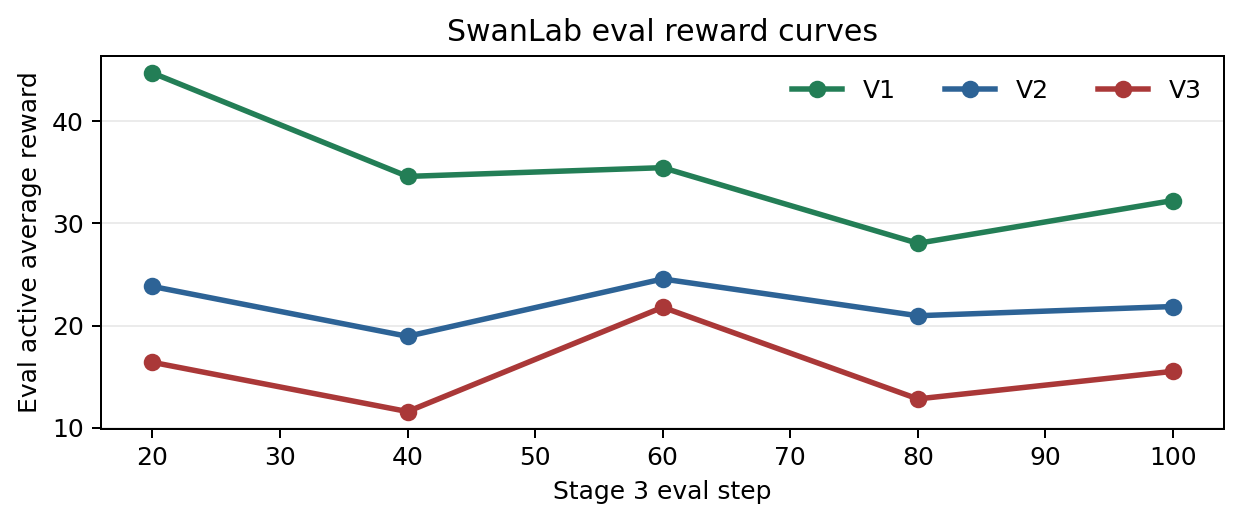
\includegraphics[width=0.88\linewidth]{assets/swanlab_reward_curve.png}
\end{figure}
\small
V1 has the strongest eval reward curve among the three Stage 3 variants.
V2/V3 add more behavior guardrails, but the reward signal becomes harder to
optimize and the final policy is less stable.
\end{frame}

\begin{frame}{V1 / V2 / V3 Ablation: Final Policies}
\begin{figure}
\centering
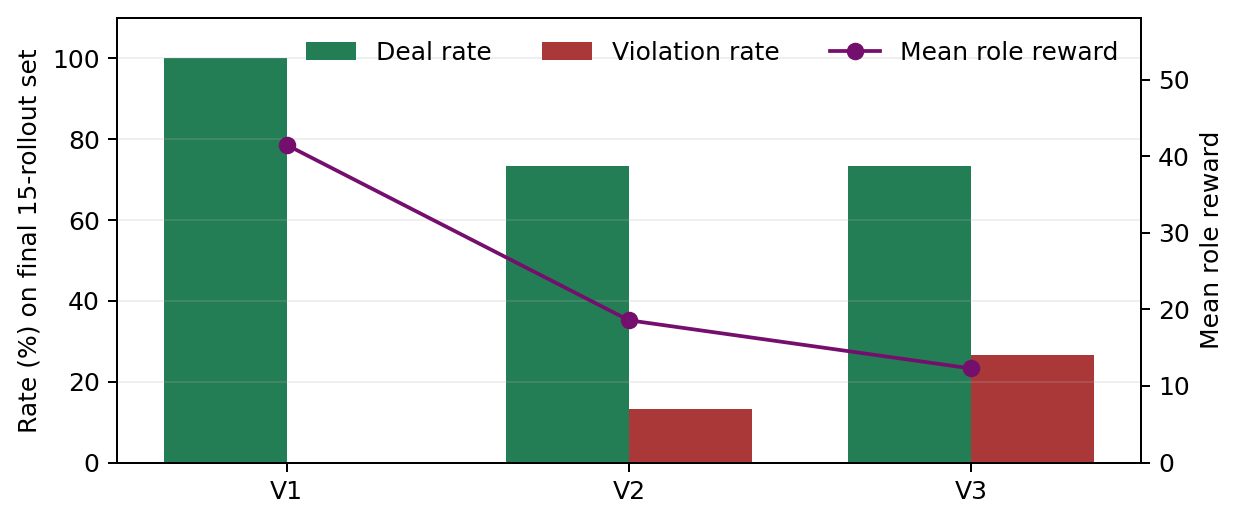
\includegraphics[width=0.88\linewidth]{assets/v123_ablation_final.png}
\end{figure}
\small
Final rollout comparison shows the trade-off clearly: V1 gives the best deal
rate and reward; V2/V3 guardrails reduce some qualitative risks but introduce
more failed or violating outcomes.
\end{frame}

\begin{frame}{Trace: A Balanced V1 Rollout}
\begin{figure}
\centering
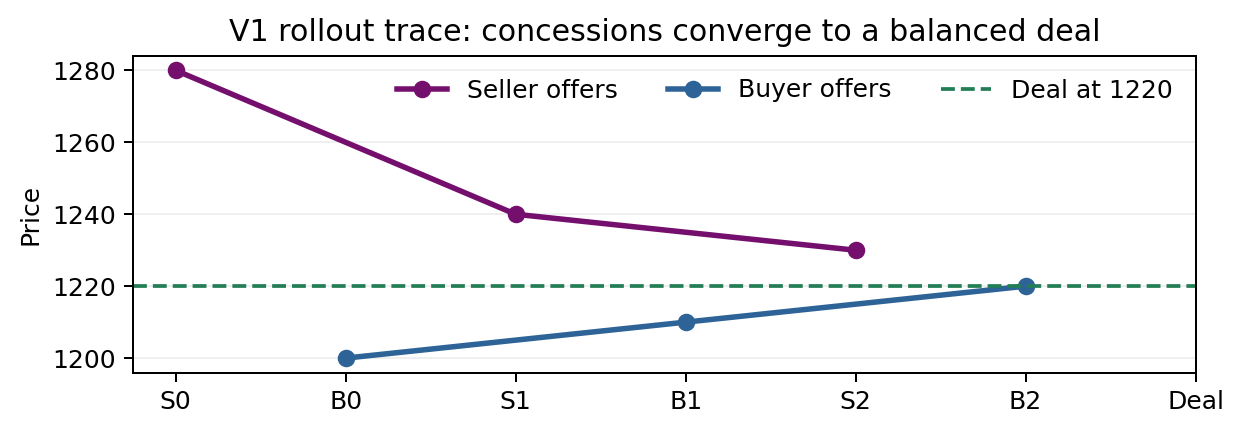
\includegraphics[width=0.88\linewidth]{assets/v1_trace_price_path.png}
\end{figure}
\small
Scenario: AirPods Pro 2. Buyer budget is 1412, seller cost is 1034, and the
deal closes at 1220. The surplus split is buyer 50.8\% and seller 49.2\%.
\end{frame}

\begin{frame}{Trace Dialogue: V1 Rollout Index 47}
\small
\begin{tabular}{@{}p{0.16\linewidth}p{0.76\linewidth}@{}}
\toprule
Seller & 1280: condition is close to new; this is already a meaningful concession.\\
Buyer & 1200: I am serious and can pay immediately if this works.\\
Seller & 1240: I can move down another step, but not much further.\\
Buyer & 1210: I can add 10 and close now.\\
Seller & 1230: final small concession.\\
Buyer & 1220: one more 10; if accepted I will buy now.\\
Seller & \texttt{<deal>1220</deal>}\\
\bottomrule
\end{tabular}
\vspace{0.15cm}
\small
This example was selected because both roles receive positive and nearly equal
reward: buyer 56.9 and seller 56.0.
\end{frame}

\section{Lessons}

\begin{frame}{What Worked, What Failed, What We Learned}
\begin{columns}
\column{0.48\linewidth}
\textbf{Worked}
\begin{itemize}
    \item SFT gave stable language and syntax.
    \item Online GRPO changed bargaining behavior.
    \item Balanced V1 produced a usable economic demo.
\end{itemize}
\column{0.48\linewidth}
\textbf{Failed / Limited}
\begin{itemize}
    \item Early Stage 3 became seller-dominant.
    \item V1 still had leakage and label residue in some samples.
    \item V2/V3 guardrails improved intent but hurt violation or deal metrics.
\end{itemize}
\end{columns}
\end{frame}

\begin{frame}{Takeaways}
\begin{itemize}
    \item The central contribution is not only the model checkpoint, but the
    environment and training loop that turn negotiation into measurable RL.
    \item Role-specific adapters are necessary because buyer and seller rewards
    are opposed even when the dialogue is shared.
    \item Reward design determines the bargaining equilibrium; stronger penalties
    are not automatically better.
    \item Next step: add human-rated dialogue quality, explicit leakage classifiers,
    and more diverse opponents.
\end{itemize}
\end{frame}

\end{document}
